\section{Results}
\label{sec:results}

\begin{table*}[t]
\centering
\caption{Final held-out Stage C results using train-only trials7 KBs, Gemini Flash, Gemini embeddings, \texttt{VALID\_NEXT\_TRIAL}, and \texttt{max\_learnings=5}. Values are mean $\pm$ std over three seeds.}
\label{tab:final-main-results}
\begin{tabular}{llrrrr}
\toprule
Environment & Framework & Tasks & Success (\%) & Score & $\Delta$ success (pp) \\
\midrule
ALFWorld & ReAct & 134 & 67.9 $\pm$ 0.0 & 0.679 $\pm$ 0.000 & \textemdash{} \\
ALFWorld & ReAct + CR & 134 & 63.9 $\pm$ 1.6 & 0.639 $\pm$ 0.016 & -4.0 $\pm$ 1.6 \\
ALFWorld & ReAct + TR & 134 & 75.4 $\pm$ 0.0 & 0.754 $\pm$ 0.000 & +7.5 $\pm$ 0.0 \\
ALFWorld & ReAct + CR + TR & 134 & \textbf{82.8 $\pm$ 0.0} & 0.828 $\pm$ 0.000 & +14.9 $\pm$ 0.0 \\
ALFWorld & Hard-neg CR + TR & 134 & 55.2 $\pm$ 0.7 & 0.552 $\pm$ 0.007 & -12.7 $\pm$ 0.7 \\
\midrule
SQL & ReAct & 200 & 91.5 $\pm$ 0.0 & 0.920 $\pm$ 0.000 & \textemdash{} \\
SQL & ReAct + CR & 200 & 88.5 $\pm$ 0.0 & 0.889 $\pm$ 0.001 & -3.0 $\pm$ 0.0 \\
SQL & ReAct + TR & 200 & 90.8 $\pm$ 0.3 & 0.917 $\pm$ 0.003 & -0.7 $\pm$ 0.3 \\
SQL & ReAct + CR + TR & 200 & \textbf{92.0 $\pm$ 0.0} & 0.922 $\pm$ 0.000 & +0.5 $\pm$ 0.0 \\
SQL & Hard-neg CR + TR & 200 & 89.5 $\pm$ 0.0 & 0.906 $\pm$ 0.000 & -2.0 $\pm$ 0.0 \\
\midrule
ScienceWorld & ReAct & 30 & \textbf{30.0 $\pm$ 8.8} & 0.214 $\pm$ 0.241 & \textemdash{} \\
ScienceWorld & ReAct + CR & 30 & 26.7 $\pm$ 3.3 & 0.171 $\pm$ 0.058 & -3.3 $\pm$ 12.0 \\
ScienceWorld & ReAct + TR & 30 & 26.7 $\pm$ 3.3 & 0.256 $\pm$ 0.086 & -3.3 $\pm$ 6.7 \\
ScienceWorld & ReAct + CR + TR & 30 & 27.8 $\pm$ 7.7 & 0.212 $\pm$ 0.134 & -2.2 $\pm$ 6.9 \\
ScienceWorld & Hard-neg CR + TR & 30 & 28.9 $\pm$ 6.9 & 0.260 $\pm$ 0.149 & -1.1 $\pm$ 15.4 \\
\bottomrule
\end{tabular}
\vspace{2pt}
{\footnotesize Score is average reward when logged; for ALFWorld ReAct, success rate is used because reward was not emitted in the final record.}
\end{table*}

\begin{table*}[t]
\centering
\caption{Final train-only KB inventory for the trials7 protocol. VNT = \texttt{VALID\_NEXT\_TRIAL}.}
\label{tab:final-kb-inventory}
\small
\resizebox{\textwidth}{!}{%
\begin{tabular}{@{}lp{0.20\linewidth}p{0.16\linewidth}cccp{0.22\linewidth}@{}}
\toprule
Environment & KB artifact & Coverage & Max trial & Memories & VNT & Audit note \\
\midrule
ALFWorld & \shortstack[l]{\texttt{alfworld\_train}\\\texttt{reflexion\_trials7}} & 115/120 observed train games & 7 & 373 & 101 & Train-only refs; no eval overlap; original 120-game manifest absent. \\
SQL & \shortstack[l]{\texttt{sql\_train\_reflexion}\\\texttt{trials7\_sanitized}} & 516/516 train tasks & 7 & 415 & 92 & Sanitized; no dev/test overlap; protocol memories quarantined. \\
ScienceWorld & \shortstack[l]{\texttt{scienceworld\_train}\\\texttt{reflexion\_trials7}\\\texttt{va80\_30cat}} & 30/30 categories, 30 variations & 7 & 129 & 34 & Train-only; 1 variation/category; failed extractions repaired. \\
\bottomrule
\end{tabular}
}
\end{table*}


\begin{figure*}[t]
\centering
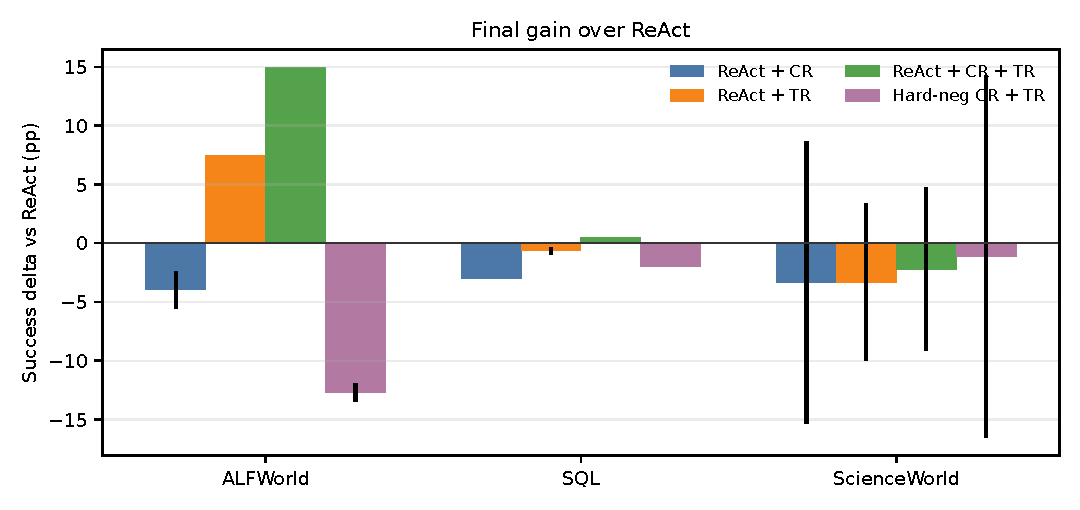
\includegraphics[width=\linewidth]{figures/final_gain_over_react.pdf}
\caption{Final success gain over ReAct for each memory variant. ALFWorld shows a clear positive CR+TR effect, SQL shows a narrow CR+TR effect, and ScienceWorld does not show a promoted positive memory result.}
\label{fig:final-gain-over-react}
\end{figure*}

\begin{figure}[t]
\centering
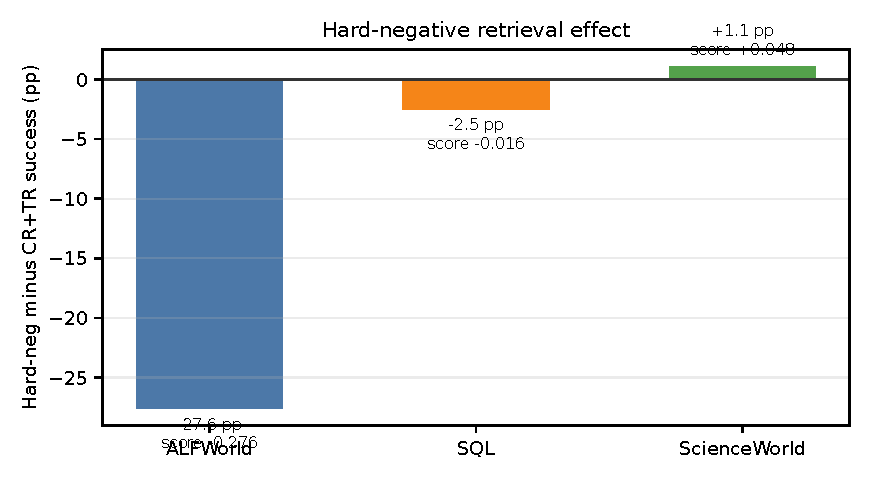
\includegraphics[width=\linewidth]{figures/final_hard_negative_effect.pdf}
\caption{Hard-negative effect in the final audits. The ALFWorld gap between CR+TR and hard-negative retrieval supports relevance as causal; the SQL and ScienceWorld gaps are smaller or unfavorable.}
\label{fig:final-hard-negative-effect}
\end{figure}

Table~\ref{tab:final-main-results} reports the final held-out Stage C results.
The headline is conditional: validated memory helps strongly in ALFWorld, weakly in SQL, and fails to promote ScienceWorld.

\subsection{ALFWorld: Positive Transfer}
\label{sec:results-alfworld}

ALFWorld is the clean positive case.
ReAct solves $67.9\%$ of the 134 validation-unseen tasks, while CR+TR solves $82.8\%$, a $+14.9$pp improvement.
TR alone is also positive ($75.4\%$, $+7.5$pp), while CR alone is negative ($63.9\%$, $-4.0$pp), showing that the two channels are useful but not automatically additive in isolation.
The combined channel is strongest, suggesting that proactive task-level context and on-demand issue-level retrieval can complement each other when the environment has reusable procedures.

The hard-negative control is decisive in ALFWorld.
Hard-negative CR+TR reaches only $55.2\%$, which is $27.6$pp below proper CR+TR and $12.7$pp below ReAct.
This rules against a simple ``extra context helps'' explanation: retrieved memory helps only when it is relevant to the task structure.

\subsection{SQL: Narrow Transfer}
\label{sec:results-sql}

SQL is a narrow-transfer diagnostic rather than a large positive result.
ReAct is already strong at $91.5\%$ success, leaving little headroom.
CR+TR improves to $92.0\%$, a small $+0.5$pp gain, but CR alone falls to $88.5\%$ and TR alone to $90.8\%$.
Hard-negative CR+TR reaches $89.5\%$, also below ReAct.

The SQL pattern indicates that some validated memories transfer, but the transfer radius is small.
Useful query repairs can be highly local to a schema, predicate, or join pattern.
This makes SQL evidence for conditional memory benefit: the best combined retrieval channel can help slightly, but individual channels and irrelevant retrievals can easily perturb a high-performing baseline.

\subsection{ScienceWorld: Diagnostic Negative Evidence}
\label{sec:results-scienceworld}

ScienceWorld should not be read as a positive transfer result.
In the final Stage C audit, ReAct is the best framework at $30.0\%$ success.
CR, TR, and CR+TR all fall below ReAct on mean success, with CR+TR at $27.8\%$.
Hard-negative CR+TR reaches $28.9\%$, matching or exceeding proper CR+TR on the headline metric.

This matters because the ScienceWorld final KB is clean but thin: it covers all 30 categories, yet only one train variation per category.
The later Phase 4.1 density gate tested whether increasing to three train variations per category would rescue the result.
It did not: same-run CR+TR underperformed ReAct on mean success and mean reward, and hard-negative retrieval matched or beat CR+TR on success in every seed.
We therefore use ScienceWorld as diagnostic evidence that memory density alone is insufficient when retrieval and validation signals do not align with reusable task structure.

\subsection{Usage, Cost, and Paired Deltas}
\label{sec:usage-deltas}

\begin{table*}[t]
\centering
\caption{Final memory usage and trajectory cost summaries from raw trajectories. Values are mean $\pm$ std over seeds.}
\label{tab:final-memory-usage}
\begin{tabular}{llrrrrr}
\toprule
Environment & Framework & Context tasks & Retrieved/task & Help calls & Help/task & Steps/task \\
\midrule
ALFWorld & ReAct & 0.0 $\pm$ 0.0 & 0.00 $\pm$ 0.00 & 0.0 $\pm$ 0.0 & 0.00 $\pm$ 0.00 & 21.00 $\pm$ 0.11 \\
ALFWorld & ReAct + CR & 132.0 $\pm$ 0.0 & 4.05 $\pm$ 0.00 & 0.0 $\pm$ 0.0 & 0.00 $\pm$ 0.00 & 28.56 $\pm$ 0.26 \\
ALFWorld & ReAct + TR & 0.0 $\pm$ 0.0 & 0.00 $\pm$ 0.00 & 302.3 $\pm$ 0.6 & 2.26 $\pm$ 0.00 & 27.69 $\pm$ 0.01 \\
ALFWorld & ReAct + CR + TR & 132.0 $\pm$ 0.0 & 4.05 $\pm$ 0.00 & 206.0 $\pm$ 0.0 & 1.54 $\pm$ 0.00 & 26.38 $\pm$ 0.01 \\
ALFWorld & Hard-neg CR + TR & 134.0 $\pm$ 0.0 & 4.67 $\pm$ 0.00 & 360.3 $\pm$ 6.4 & 2.69 $\pm$ 0.05 & 34.72 $\pm$ 0.08 \\
\midrule
SQL & ReAct & 0.0 $\pm$ 0.0 & 0.00 $\pm$ 0.00 & 0.0 $\pm$ 0.0 & 0.00 $\pm$ 0.00 & 8.67 $\pm$ 0.00 \\
SQL & ReAct + CR & 178.0 $\pm$ 0.0 & 2.05 $\pm$ 0.00 & 0.0 $\pm$ 0.0 & 0.00 $\pm$ 0.00 & 8.94 $\pm$ 0.00 \\
SQL & ReAct + TR & 0.0 $\pm$ 0.0 & 0.00 $\pm$ 0.00 & 23.0 $\pm$ 0.0 & 0.12 $\pm$ 0.00 & 9.23 $\pm$ 0.00 \\
SQL & ReAct + CR + TR & 178.0 $\pm$ 0.0 & 2.05 $\pm$ 0.00 & 20.0 $\pm$ 0.0 & 0.10 $\pm$ 0.00 & 9.11 $\pm$ 0.01 \\
SQL & Hard-neg CR + TR & 171.7 $\pm$ 0.6 & 1.68 $\pm$ 0.01 & 24.0 $\pm$ 0.0 & 0.12 $\pm$ 0.00 & 9.03 $\pm$ 0.00 \\
\midrule
ScienceWorld & ReAct & 0.0 $\pm$ 0.0 & 0.00 $\pm$ 0.00 & 0.0 $\pm$ 0.0 & 0.00 $\pm$ 0.00 & 30.96 $\pm$ 1.67 \\
ScienceWorld & ReAct + CR & 30.0 $\pm$ 0.0 & 4.40 $\pm$ 0.00 & 0.0 $\pm$ 0.0 & 0.00 $\pm$ 0.00 & 30.48 $\pm$ 1.24 \\
ScienceWorld & ReAct + TR & 0.0 $\pm$ 0.0 & 0.00 $\pm$ 0.00 & 37.3 $\pm$ 6.4 & 1.24 $\pm$ 0.21 & 34.19 $\pm$ 2.13 \\
ScienceWorld & ReAct + CR + TR & 30.0 $\pm$ 0.0 & 4.40 $\pm$ 0.00 & 20.7 $\pm$ 3.8 & 0.69 $\pm$ 0.13 & 31.23 $\pm$ 1.99 \\
ScienceWorld & Hard-neg CR + TR & 30.0 $\pm$ 0.0 & 4.17 $\pm$ 0.00 & 31.3 $\pm$ 2.1 & 1.04 $\pm$ 0.07 & 33.08 $\pm$ 0.37 \\
\bottomrule
\end{tabular}
\end{table*}

\begin{table*}[t]
\centering
\caption{Paired task-level deltas against ReAct on the final held-out Stage C runs. Values are mean $\pm$ std over seeds.}
\label{tab:final-paired-deltas}
\resizebox{\textwidth}{!}{%
\begin{tabular}{llrrrrr}
\toprule
Environment & Framework & Common tasks & $\Delta$ success (pp) & $\Delta$ score & Improved & Regressed \\
\midrule
ALFWorld & ReAct + CR & 134 $\pm$ 0 & -4.0 $\pm$ 1.6 & \textemdash{} & 20.3 $\pm$ 1.5 & 25.7 $\pm$ 0.6 \\
ALFWorld & ReAct + TR & 134 $\pm$ 0 & +7.5 $\pm$ 0.0 & \textemdash{} & 27.0 $\pm$ 0.0 & 17.0 $\pm$ 0.0 \\
ALFWorld & ReAct + CR + TR & 134 $\pm$ 0 & +14.9 $\pm$ 0.0 & \textemdash{} & 33.0 $\pm$ 0.0 & 13.0 $\pm$ 0.0 \\
ALFWorld & Hard-neg CR + TR & 134 $\pm$ 0 & -12.7 $\pm$ 0.7 & \textemdash{} & 18.7 $\pm$ 0.6 & 35.7 $\pm$ 0.6 \\
\midrule
SQL & ReAct + CR & 200 $\pm$ 0 & -3.0 $\pm$ 0.0 & -0.031 $\pm$ 0.001 & 2.0 $\pm$ 0.0 & 8.0 $\pm$ 0.0 \\
SQL & ReAct + TR & 200 $\pm$ 0 & -0.7 $\pm$ 0.3 & -0.003 $\pm$ 0.003 & 2.0 $\pm$ 0.0 & 3.3 $\pm$ 0.6 \\
SQL & ReAct + CR + TR & 200 $\pm$ 0 & +0.5 $\pm$ 0.0 & 0.002 $\pm$ 0.000 & 3.0 $\pm$ 0.0 & 2.0 $\pm$ 0.0 \\
SQL & Hard-neg CR + TR & 200 $\pm$ 0 & -2.0 $\pm$ 0.0 & -0.014 $\pm$ 0.000 & 2.0 $\pm$ 0.0 & 6.0 $\pm$ 0.0 \\
\midrule
ScienceWorld & ReAct + CR & 30 $\pm$ 0 & -3.3 $\pm$ 12.0 & -0.043 $\pm$ 0.284 & 2.7 $\pm$ 1.2 & 3.7 $\pm$ 2.5 \\
ScienceWorld & ReAct + TR & 30 $\pm$ 0 & -3.3 $\pm$ 6.7 & 0.042 $\pm$ 0.240 & 3.0 $\pm$ 1.0 & 4.0 $\pm$ 1.0 \\
ScienceWorld & ReAct + CR + TR & 30 $\pm$ 0 & -2.2 $\pm$ 6.9 & -0.002 $\pm$ 0.148 & 2.0 $\pm$ 1.0 & 2.7 $\pm$ 1.2 \\
ScienceWorld & Hard-neg CR + TR & 30 $\pm$ 0 & -1.1 $\pm$ 15.4 & 0.046 $\pm$ 0.354 & 4.3 $\pm$ 1.5 & 4.7 $\pm$ 3.2 \\
\bottomrule
\end{tabular}
}
\end{table*}


\begin{figure*}[t]
\centering
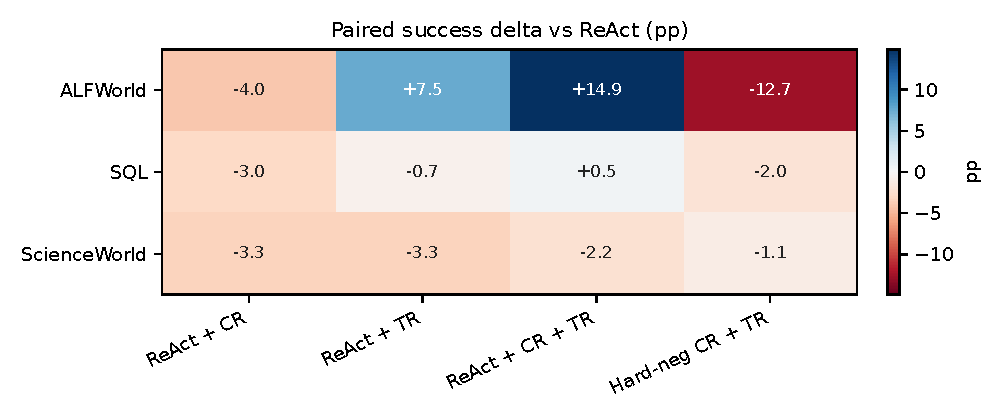
\includegraphics[width=\linewidth]{figures/final_paired_delta_heatmap.pdf}
\caption{Paired task-level deltas against ReAct. Positive and negative cells expose where memory helps, regresses, or remains neutral under matched task comparisons.}
\label{fig:final-paired-delta-heatmap}
\end{figure*}

\begin{figure}[t]
\centering
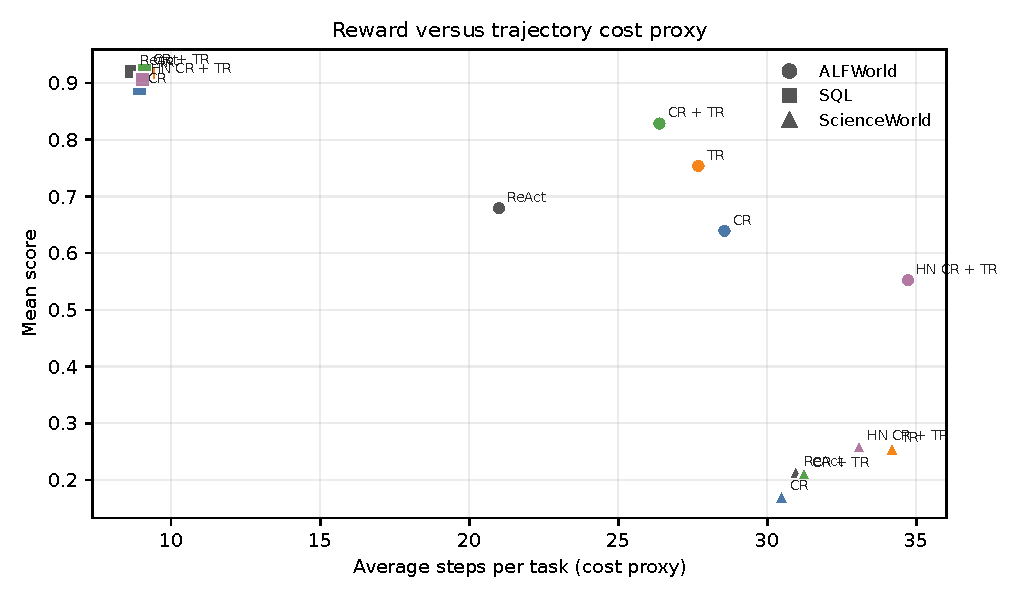
\includegraphics[width=\linewidth]{figures/final_reward_vs_cost.pdf}
\caption{Final score versus trajectory cost, using average steps per task as a cost proxy because provider dollar cost is unavailable in the final raw logs.}
\label{fig:final-reward-vs-cost}
\end{figure}

Table~\ref{tab:final-memory-usage} shows that retrieval was active in the memory variants and that trajectory cost changes differ by environment.
ALFWorld CR+TR uses both context memories and help calls while remaining far below the hard-negative variant in steps per task.
SQL retrieval is sparse, especially for TR, consistent with its narrow-transfer character.
ScienceWorld retrieval occurs reliably, but usage does not translate into better success.

Table~\ref{tab:final-paired-deltas} and Figure~\ref{fig:final-paired-delta-heatmap} sharpen the same picture at the task level.
ALFWorld CR+TR improves many more tasks than it regresses.
SQL CR+TR has only a small favorable imbalance.
ScienceWorld has unstable paired deltas with no promoted CR+TR advantage.
